\documentclass{beamer}

\usepackage[utf8]{inputenc}
\usepackage[T1]{fontenc}
\usepackage[english]{babel}
\usepackage{lmodern}
\usepackage{color}
\usepackage{fix-cm}
\usepackage{textpos}
\usepackage{eurosym}
\usepackage{multirow}
\usepackage{perpage}
\usepackage{eso-pic}
\usepackage{times}
\usepackage{tikz}
\usetikzlibrary{matrix}

\colorlet{helpful}{lime!40}
\colorlet{harmful}{red!30}
\colorlet{internal}{yellow!20}
\colorlet{external}{cyan!30}
\colorlet{S}{helpful!50!internal}
\colorlet{W}{harmful!50!internal}
\colorlet{O}{helpful!50!external}
\colorlet{T}{harmful!50!external}

\newcommand{\texta}{Positif\par}
\newcommand{\textb}{Négatif\par}
\newcommand{\textcn}{Interne\par}
\newcommand{\textdn}{Externe\par}

\newcommand{\back}[1]{\fontsize{80}{70}\selectfont #1}
%%%

\graphicspath{{images/}}

\newcommand{\placetextbox}[3]{% \placetextbox{<horizontal pos>}{<vertical pos>}{<stuff>}
	\setbox0=\hbox{#3}% Put <stuff> in a box
	\AddToShipoutPictureFG*{% Add <stuff> to current page foreground
		\put(\LenToUnit{#1\paperwidth},\LenToUnit{#2\paperheight}){\vtop{{\null}\makebox[0pt][c]{#3}}}%
	}%
}%

% Redéfinis les marges des tableaux
\let\oldtabular=\tabular
\def\tabular{\small\oldtabular}
\renewcommand{\arraystretch}{1.5}

\usetheme{Warsaw}
\usecolortheme{orchid}

% Permet de réinitialiser les footnote à chaque frame. Nécéssite 2 compilations.
\MakePerPage{footnote}

\setlength{\TPHorizModule}{0.01\textwidth}
\setlength{\TPVertModule}{0.01\textheight}

\setbeamertemplate{navigation symbols}{}

\title[Dawwyd]{Dawwyd\\Reconnaissance Vocale}

\author[HOUDAYER \and RUHIER]{
	Benoit HOUDAYER\\
    \and
	Anthony RUHIER
}
\institute[GE75 - UTBM]{
    Gestion de Projet (SI75)\\Université de Technologie Belfort--Montbéliard}
\date{Février 2016}

\begin{document}

% Permet de masquer le comptage de slides
\bgroup
\makeatletter
\setbeamertemplate{headline}{}
\setbeamertemplate{footline}
{
  \leavevmode%
  \hbox{%
  \begin{beamercolorbox}[wd=.5\paperwidth,ht=2.25ex,dp=1ex,center]{title in head/foot}%
    \usebeamerfont{title in head/foot}\insertshorttitle
  \end{beamercolorbox}%
  \begin{beamercolorbox}[wd=.5\paperwidth,ht=2.25ex,dp=1ex,center]{date in head/foot}%
    \usebeamerfont{date in head/foot}\insertshortdate{}
%    \insertframenumber{} / \inserttotalframenumber\hspace*{2ex}
  \end{beamercolorbox}}%
}
\makeatother

\begin{frame}[noframenumbering]
 	\frametitle{}
	\titlepage
	\hfill
\includegraphics[height=1cm]{logo-utbm.eps}\hspace*{-1em}
\end{frame}
\egroup

\logo{
\includegraphics[height=1cm]{images/logo-utbm.eps}\hspace*{2em}}


% Ajout du compteur de slides
\expandafter\def\expandafter\insertshorttitle\expandafter{%
      \insertshorttitle\hfill%
      \insertframenumber\,/\,\inserttotalframenumber}

\begin{frame}
	\begin{small}
	\frametitle{Plan}
	\tableofcontents
	\end{small}
\end{frame}


%%%% Includes des sections :
%%%%%%%%%%%%%%%%%%%%%%%%%%%%%%
%
\section{Répondre à un problème quotidien}

\subsection{Types de tâches}
\begin{frame}
\frametitle{Tâches secondaires}
\begin{itemize}
    \setlength\itemsep{2em}
	\item Écoute de musique
	\item Consultation des actualités/météo
	\item Réseaux sociaux
\end{itemize}

\end{frame}

\begin{frame}
\frametitle{Tâches intrusives}
\begin{itemize}
    \setlength\itemsep{2em}
    \item Écoute de musique $\rightarrow$ ouvrir le lecteur
    \item Éonsultation des actualités/météo $\rightarrow$ ouvrir le navigateur
    \item Ééseaux sociaux $\rightarrow$ lire les messages des gens
\end{itemize}
\end{frame}

\section{Planification}

\subsection{WBS}
\begin{frame}
\begin{center}
\begin{columns}
\begin{column}{330px}
{
    \begin{figure}[h!]
        \centering
        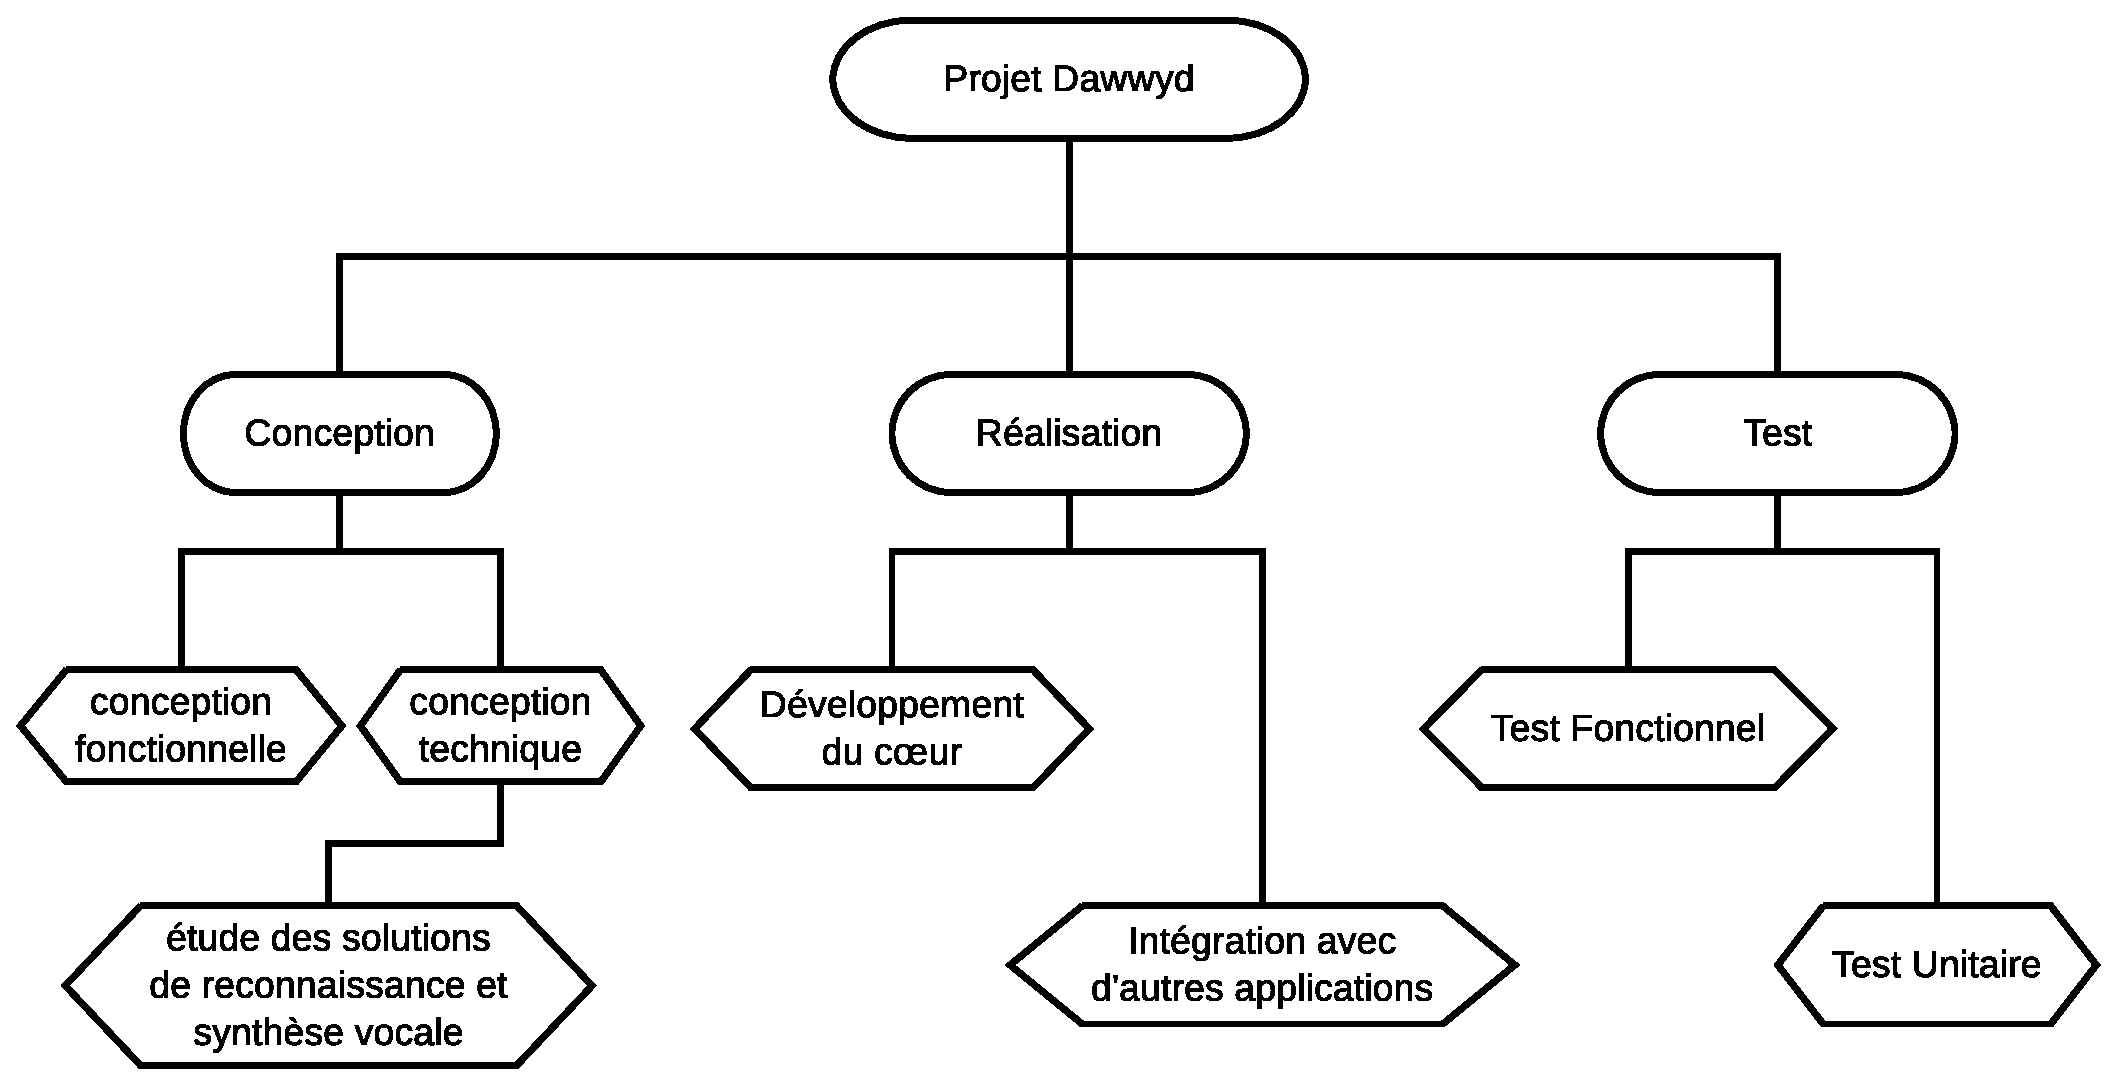
\includegraphics[width=300px]
            {images/WBS}
        \caption{WBS}
    \end{figure}
}
\end{column}
\end{columns}
\end{center}
\end{frame}


\subsection{Cahier des charges}
\begin{frame}
\frametitle{Cahier des charges}
\begin{itemize}
    \setlength\itemsep{1.5em}
    \item Synthétiser la voix de l'utilisateur sous forme de texte
    \item Lien entre les données textuelles et fonctions implémentées
    \item S'intégrer avec les applications de l'utilisateur
    \item Intégration facile de nouvelles applications
    \item Communiquer avec l'utiliser via la synthèse vocale
\end{itemize}
\end{frame}


\subsection{Diagramme de PERT et matrice SWOT}
{
\logo{}
\begin{frame}
\begin{center}
\begin{columns}
\begin{column}{330px}
{
    \vspace{-0.5em}
    \begin{figure}[h!]
        \centering
        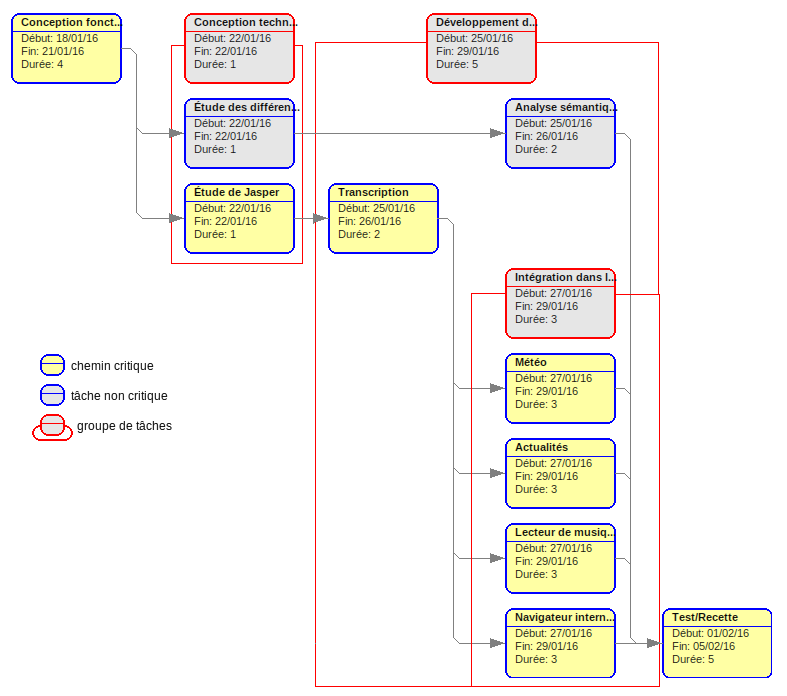
\includegraphics[height=210px]
            {images/pert}
        \vspace{-1em}
        \caption{PERT}
    \end{figure}
}
\end{column}
\end{columns}
\end{center}
\end{frame}
}


\begin{frame}[fragile]{Examples}
\frametitle{Matrice SWOT}
\begin{center}
	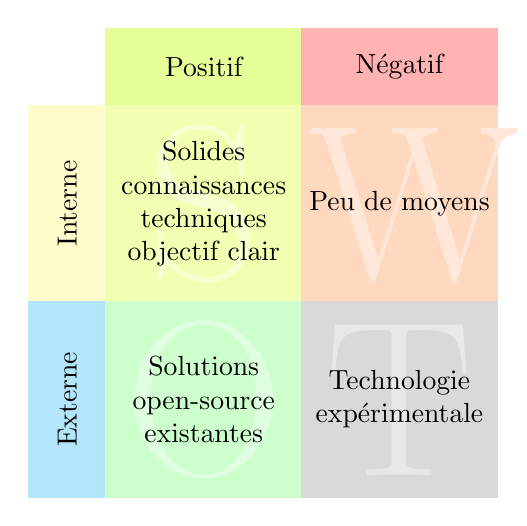
\begin{tikzpicture}[
	any/.style={minimum width=2.5cm,minimum height=2.5cm,%
		text width=2.3cm,align=center,outer sep=0pt},
	header/.style={any,minimum height=1cm,fill=black!10},
	leftcol/.style={header,rotate=90},
	mycolor/.style={fill=#1, text=#1!60!white}
	]

	\matrix (SWOT) [matrix of nodes,nodes={any,anchor=center},%
	column sep=-\pgflinewidth,%
	row sep=-\pgflinewidth,%
	row 1/.style={nodes=header},%
	column 1/.style={nodes=leftcol},%
	inner sep=0pt]%
	{
		&|[fill=helpful]| {\texta} & |[fill=harmful]| {\textb} \\
		|[fill=internal]| {\textcn} & |[mycolor=S]| \back{S} & |[mycolor=W]| \back{W} \\
		|[fill=external]| {\textdn} & |[mycolor=O]| \back{O} & |[mycolor=T]| \back{T} \\
	};

    \node[any, anchor=center] at (SWOT-2-2) {Solides connaissances techniques\\objectif clair};
	\node[any, anchor=center] at (SWOT-2-3) {Peu de moyens};
	\node[any, anchor=center] at (SWOT-3-2) {Solutions open-source existantes};
	\node[any, anchor=center] at (SWOT-3-3) {Technologie expérimentale};
	\end{tikzpicture}
\end{center}
\end{frame}


\section{Recettes et améliorations}

\subsection{Recette}
\begin{frame}
\frametitle{Recette}
\begin{itemize}
    \setlength\itemsep{2em}
    \item Toutes les fonctions prévues implémentées
    \item Reconnaissance vocale, lecture du texte, gestion du français
    \item Plugin de lecture de musique, météo, lancement d'applications
    \item Pas de retard dans le planning
\end{itemize}
\end{frame}


\subsection{Diagramme de Gantt}

\begin{frame}
\frametitle{Diagramme de Gantt}
	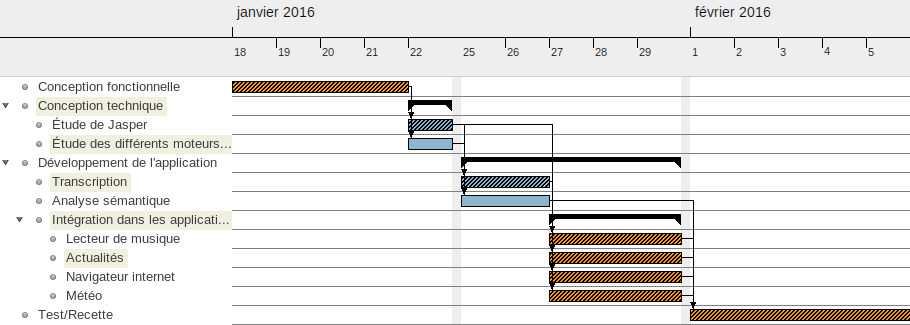
\includegraphics[width=11cm]{gantt}
\end{frame}

\begin{frame}
\frametitle{Des questions ?}
\centering
\begin{figure}
    
\includegraphics[height=5cm]{hal_dawwyd}
    \caption{Dawwyd vous écoute}
\end{figure}
\end{frame}

\end{document}
